\part*{ЗАКЛЮЧЕНИЕ}
\addcontentsline{toc}{part}{\textbf{ЗАКЛЮЧЕНИЕ}} 

Обнаружение синтезированного звука - довольно сложная задача, и для успешного решения требуется значительное внимание. Как предложено во многих исследованиях по обнаружению синтетического звука, наилучшим вариантом классификации звука в настоящее время являются глубокие нейронные сети.

На рисунке (\ref{fig:deep-classification}) представлено, класификации методов обнаружения синтетического звука: 
\begin{figure}[H]
	\centering
	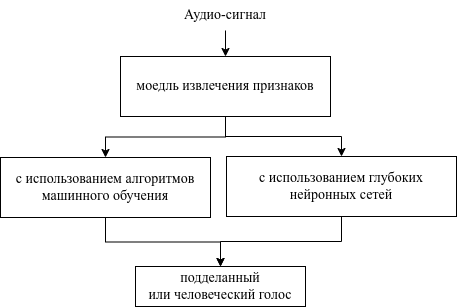
\includegraphics[width=0.5\linewidth]{images/method-classification.png}
	\caption{Класификации методов обнаружения синтетического звука}
	\label{fig:deep-classification}
\end{figure}

Структура работы системы обнаружения синтетического звука может быть описана следующим образом:

\begin{enumerate}
    \item На вход поступает аудиозапись.
    \item Модель извлечения признаков предварительно обрабатывает запись.
    \item Затем происходит процесс извлечения признаков.
    \item Модель классификации использует эти признаки для обучения и распознавания.
\end{enumerate}

Значительную роль в эффективности работы модели играют признаки, передаваемые в модель для классификации, а также сам процесс работы модели классификации.

Следует отметить, что огромное значение для работоспособности и результатов модели по классификации имеют корпусы данных, используемые для обучения и извлечение признаков, которое обнаруживается в процессе обучения модели.